\documentclass[compress]{beamer}
%\documentclass[handout]{beamer}

% for themes, etc.
\mode<presentation> { \usetheme{Boxes} }
\usecolortheme{whale}
\usecolortheme{orchid}
\useoutertheme{split}
\useinnertheme[shadow]{rounded}
%\setbeameroption{show notes}

\usepackage{times}  % fonts are up to you
\usepackage{graphicx}
\usepackage{amsbsy,amsmath,amsthm,amssymb,times,graphicx}
\usepackage{natbib}
\usepackage{bm}
%\usepackage[longnamesfirst,sort]{natbib}
%\newcommand{\pcite}[1]{\citeauthor{#1}'s \citeyearpar{#1}}

\newcommand {\pp} {\vspace{3 mm}}
\newcommand {\ppp} {\vspace{5 mm}}
\newcommand {\bpi} {{\color{blue} \pi}}
\newcommand {\sse} {\sigma^2_e}
\newcommand {\sst} {\sigma^2_\theta}
\newcommand {\ssq} {{\bf \sigma}^2}
\newcommand {\bth} {\boldsymbol{\theta}}
\newcommand {\sts} {\mathsf{Y}}
\newcommand {\say} {{\cal B}(\mathsf{Y})}
\newcommand {\nn} {\mathbb{N}}
\newcommand {\bla} {\boldsymbol{\lambda}}
\newcommand {\lae} {\lambda_e}
\newcommand {\lat} {\lambda_\theta}
\newcommand {\ybi} {\overline{y}_i}
\newcommand {\tb} {\overline{\theta}}
\newcommand {\Var} {\text{Var}}
\newcommand {\Cov} {\text{Cov}}
\newcommand {\E} {\text{E}}
\newcommand {\last} {last}
\newcommand {\con} {\text{const.}}
\newcommand {\z} {\boldsymbol{z}}
\newcommand {\bzeta} {\boldsymbol{\xi}}
\newcommand {\bV} {{\bf V}}
\newcommand {\bL} {{\bf L}}
\newcommand {\M} {{\bf M}}
\newcommand {\B} {{\bf B}}
\newcommand {\X} {{\bf X}}
\newcommand {\m} {{\bf m}}
\newcommand {\sX} {{\cal X}}
\newcommand{\red}[1]{{\color{red}{#1} }}
\newcommand{\blue}[1]{{\color{blue}{#1} }}
\newcommand{\bb} {\bm{\beta}}
\newcommand{\bs} {\bm{\Sigma}}
\newcommand{\by} {\bm{Y}}
\newcommand{\bya} {\bm{Y_1}}
\newcommand{\byk} {\bm{Y_K}}
\newcommand{\bxa} {\bm{X_1}}
\newcommand{\bxp} {\bm{X_p}}
\newcommand{\bx} {\bm{x}}
\newcommand{\bxi} {\bm{x_i}}
\newcommand{\bX} {\bm{X}}
\newcommand{\bmk} {\bm{\mu_k}}
\newcommand{\bmka} {\bm{\mu_{k_1}}}
\newcommand{\bmkb} {\bm{\mu_{k_2}}}
\newcommand{\ba} {\bm{a}}
\newcommand{\baa} {\bm{a_1}}
\newcommand{\bak} {\bm{a_k}}
\newcommand{\bab} {\bm{a_2}}
\newcommand{\bxpp} {\bm{x^{''}}}
\newcommand{\bxap} {\bm{x_1^{'}}}
\newcommand{\bxbp} {\bm{x_2^{'}}}
\newcommand{\bxapp} {\bm{x_1^{''}}}
\newcommand{\bxbpp} {\bm{x_2^{''}}}
\newcommand{\bxkpp} {\bm{x_k^{''}}}
\newcommand{\bmkh} {\bm{\hat{\mu_k}}}
\title[Chapter 4: Linear Methods for Classification]{{\large Chapter 4: Linear Methods for Classification\newline Sections 4.1-4.3}}

\author[Rebecca Steorts]{Rebecca Steorts\\{\hfill} }

\institute[UF]{Department of Statistics \\
    University of Florida\\
{\hfill}\\Statistical Learning}
\date{February 1, 2010}

\begin{document}

%\bibliographystyle{ims}
%\bibliography{refs}

\begin{frame}
\titlepage
\end{frame}

\begin{frame}{Outline}
\tableofcontents
\end{frame}

\section[Introduction]{Introduction}
\subsection[Linear Methods]{General Setup}


\note{I can have notes in here of what I'm going to talk about.}


\frame{
\frametitle{General Setup} 

Response categories are coded as an indicator variable. Suppose $\mathcal{G}$ has $K$ classes, then $\bya$ is a vector of 0's and 1's indicating for example whether each person is in class 1. \\
\begin{itemize}
\item The indicator response matrix is defined as $Y = (\bya, \ldots, \byk).$
\item $Y$ is a matrix of 0's and 1's with each row having a single 1 indicating a person is in class $k.$
\item The $i^{\text{th}}$ person of interest has covariate values $\bm{x_{i1}},\ldots,\bm{x_{ip}}$ that will be represented by $X_{N\times p}.$
\item Our goal is to predict what class each observation is in given its covariate values. 
\end{itemize}
}



\section[Regression]{Linear Regression}
\subsection{Naive Method}

\frame{
\frametitle{Linear Regression of an Indicator Matrix} 
\begin{itemize}
\item Let's proceed blindly and use a naive method of linear regression.
\item Fit a linear regression to each column of Y.
\item The coefficient matrix is $\hat{B} = (X'X)^{-1}X'Y$.
\item $\hat{Y} = X(X'X)^{-1}X'Y$
\item The $k^{th}$ column of $\hat{B}$ contains the estimates corresponding to the linear regression coefficients that we get from regressing $\bxa,\ldots,\bxp$ onto $\byk$.


\end{itemize}
}



\frame{
\frametitle{Linear Regression of an Indicator Matrix}  

Look at $\hat{Y}$ corresponding to the indicator variable for each class $k.$ Assign each person to the class for which $\hat{Y}$ is the largest.\newline

More formally stated, a new observation with covariate $\bm{x}$ is classified as follows: 
\begin{itemize}
\item Compute the fitted output $\bm{\hat{Y}_{new}}(\bx) = [(1, \bx)' \hat{B}]'$.
\vspace{0.3cm}
\item Identify the largest component of $\bm{\hat{Y}_{new}}(\bx)$ and classify according to \begin{displaymath}\hat{G}(\bx) = \text{arg} \max_k  \bm{\hat{Y}_{new}}(\bx).\end{displaymath} 

\end{itemize}
}


\frame{
\frametitle{Does this Approach Make Sense?} 

\begin{itemize}
\item The regression line estimates $\text{E}(Y_k|\bX=\bx) = \text{P}(G=k|\bX=\bx)$ so the method seems somewhat sensible at first.
\item Although $\sum_k \hat{Y}_k(\bx) = 1$ for any $\bx$ as long as there is an intercept in the model (exercise), $\hat{Y}_k(\bx)$ can be negative or greater than 1 which is nonsensical to the initial problem statement. 
\item Worse problems can occur when classes are masked by others due to the rigid nature of the regression model.

\end{itemize}
}


\subsection{Iris Example}

\frame{
\frametitle{Iris Data} 
\begin{itemize}
\item This data set (Fisher, Annals of Eugenics,1936) gives the measurements of sepal and petal length and width for 150 flowers using 3 species of iris (50 flowers per species). 
\item The species considered are setosa, versicolor, and virginica. 
\item To best illustrate the methods of classification, we considered how petal width and length predict the species of a flower. 
\end{itemize}
}

\frame{
\frametitle{Iris Data} 


\vspace{-0.4cm}
\begin{table}[htdp]
\begin{center}
%\hspace*{-0.3cm}
\begin{tabular}{c|c|c|c|c}

Sepal L	&	Sepal W	&	Petal L	&	Petal W	&	Species	\\ \hline 
5.1	&	3.5	&	1.4	&	0.2	&	setosa	\\ 
4.9	&	3.0	&	1.4	&	0.2	&	setosa	\\ 
4.7	&	3.2	&	1.3	&	0.2	&	setosa	\\ \
$\vdots$	&	$\vdots$	&	$\vdots$	&	$\vdots$	&	$\vdots$	\\ 
7.0	&	3.2	&	4.7	&	1.4	&	versicolor	\\ 
6.4	&	3.2	&	4.5	&	1.5	&	versicolor	\\ 
6.9	&	3.1	&	4.9	&	1.5	&	versicolor	\\ 
$\vdots$	&	$\vdots$	&	$\vdots$	&	$\vdots$	&	$\vdots$	\\ 
6.3	&	3.3	&	6.0	&	2.5	&	virginica	\\ 
5.8	&	2.7	&	5.1	&	1.9	&	virginica	\\ 
7.1	&	3.0	&	5.9	&	2.1	&	virginica	\\ 
\end{tabular}
\end{center}
\label{default}
\end{table}



}


\frame{
\frametitle{Illustration of Masking Effect} 
\vspace{-.7cm}
\begin{center}
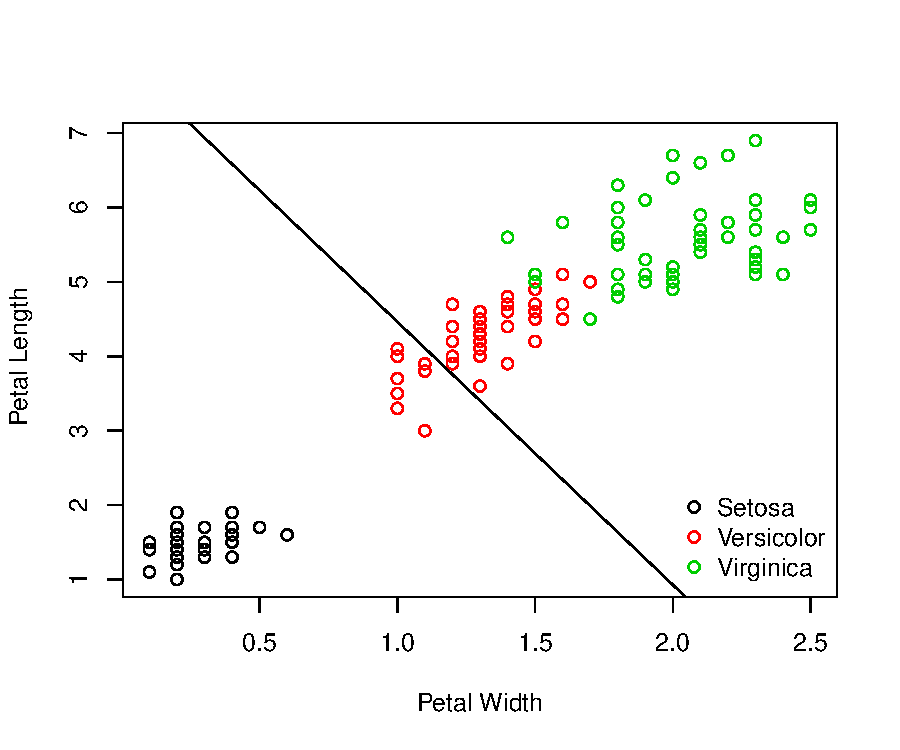
\includegraphics[width = 0.9\textwidth]{linear.pdf}
\end{center}

}

\frame{
\frametitle{Illustration of Masking Effect} 


To recap the previous picture, we can see that using linear regression to predict for different classes can lead to a masking effect of one group or more. This occurs for the following reasons:
\begin{enumerate}
\item There is a plane that is high in the bottom left corner (setosa) and low in the top right corner (virginica).
\item There is a second plane that is high in the top right corner (virginica) but low in the bottom left corner (setosa).
\item The third plane is approximately flat since it tries to linearly fit a collection of points that is high in the middle (versicolor) and low on both ends.
\end{enumerate}

}

\section{LDA}
\subsection{Assumptions}

\frame{
\frametitle{LDA Model Assumptions} 

For each person, conditional on them being in class $k$, we assume 
$\bX|G = k \sim N_p(\bmk, \Sigma_k).$ That is,

$$f_k(\bx) = \frac{1}{(2\pi)^{p/2}|\Sigma_k|^{1/2}}\exp{\left\{-\frac{1}{2}(\bx-\bmk)'\Sigma_k^{-1}(\bx-\bmk)\right\}}.$$
\vspace{0.3cm}

Linear Discriminant Analysis (LDA) assumes $\Sigma_k = \Sigma$ for all $k.$ 
 


}





\frame{
\frametitle{LDA Model Assumptions} 

In practice the parameters of the Gaussian distribution are unknown and must be estimated by:
\begin{itemize}
\item $\hat{\pi_k} = N_k/ N$, where $N_k$ is the number of people of class $k$
\item $\hat{\bmk} = \sum_{i: g_i = k} \bxi/N_k$
\item $\hat{\Sigma} = \sum_{k=1}^K \sum_{i: g_i = k} (\bxi - \hat{\bmk})(\bxi - \hat{\bmk})'/(N-K),$

\end{itemize}
\vspace{0.3cm}
 where $\pi_k = P(G = k).$

}


\subsection{Derivations}
\frame{

\frametitle{Derivations} 

We're interested in computing

$$P(G = k | \bX = \bx) = \frac{P (G = k, \bX = \bx)} {P(\bX = \bx)} $$
$$ = \frac{P (\bX= \bx | G = k) P(G = k)} {\sum_{k=1}^K P(\bX=\bx, G=k)}$$
$$ = \frac{f_k(\bx) \pi_k}{\sum_{j=1}^K f_j(\bx) \pi_j}. $$






}

\frame{
\frametitle{Derivations} 
We will compute $P(G=k|\bX=\bx)$ for each class $k.$ \newline

Consider comparing $P(G = k_1 | \bX=\bx)$ and $P(G = k_2 | \bX=\bx).$

Then
$$ \log\bigg[\frac{P(G = k_1 | \bX=\bx)}{ P(G = k_2 | \bX=\bx)}\bigg] = \log\bigg[      
\frac{f_{k_1}(\bx) \pi_{k_1} }{ f_{k_2}(\bx) \pi_{k_2}} \bigg]$$

$$  \hspace{-0.4cm}=-\frac{1}{2}(\bx-\bmka)'\Sigma^{-1}(\bx-\bmka) + \frac{1}{2}(\bx-\bmkb)'\Sigma^{-1}(\bx-\bmkb)+ \log\left[\frac{\pi_{k_1}}{ \pi_{k_2}}\right]$$
$$ = (\bmka - \bmkb)'\Sigma^{-1}\bx - \frac{1}{2}\bmka'\Sigma^{-1}\bmka  + \frac{1}{2}\bmkb' \Sigma^{-1} \bmkb + \log\bigg[\frac{\pi_{k_1}}{ \pi_{k_2}}\bigg] $$
}



\frame[containsverbatim]{
\frametitle{Derivations} 

Now let's consider the boundary between predicting someone to be in class $k_1$ or class $k_2.$ To be on the the boundary, we must decide what $\bx$ would need to be if we think that a person is equally likely to be in class $k_1$ or $k_2.$ \newline 

This reduces to solving
$$ (\bmka - \bmkb)'\Sigma^{-1}\bx -\frac{1}{2} \bmka'\Sigma^{-1}\bmka  + \frac{1}{2}\bmkb' \Sigma^{-1} \bmkb + \log\bigg[\frac{\pi_{k_1}}{ \pi_{k_2}}\bigg]  = 0,$$\vspace{-.5cm}

which is linear in $\bx.$ 

\begin{itemize}
\item The boundary will be a line for two dimensional problems.
\item The boundary will be a hyperplane for three dimensional problems.


\end{itemize}

}

\frame[containsverbatim]{
\frametitle{Derivations} 
The linear log-odds function implies that our decision boundary between classes $k_1$ and $k_2$ will be the set where $$P(G = k_1|\bX=\bx) = P(G= k_2|\bX=\bx),$$ which is linear in $\bx.$ In $p$ dimensions, this is a hyperplane. \newline

We can then say that class $k_1$ is more likely than class $k_2$ if $$P(G = k_1|\bX=\bx) > P(G= k_2|\bX=\bx) \implies$$
$$\log\bigg[\frac{P(G = k_1|\bX=\bx)}{  P(G= k_2|\bX=\bx)} \bigg] > 0 \implies$$

}






\frame{
\frametitle{Derivations} 
\vspace{-.6cm}
$$ (\bmka - \bmkb)'\Sigma^{-1}\bx -\frac{1}{2} \bmka'\Sigma^{-1}\bmka  +\frac{1}{2} \bmkb' \Sigma^{-1} \bmkb + \log\bigg[\frac{\pi_{k_1}}{ \pi_{k_2}}\bigg]> 0 \implies$$ 
\vspace{-.2cm}
$$\hspace{-.4cm} \bmka'\Sigma^{-1}\bx - \frac{1}{2}\bmka'\Sigma^{-1}\bmka + \log(\pi_{k_1}) >
\bmkb'\Sigma^{-1}\bx - \frac{1}{2}\bmkb'\Sigma^{-1}\bmkb + \log(\pi_{k_2}).
$$

\begin{block}{Definition}
The linear discriminant function $\delta_k^L(\bx)$ is defined as
$$ \delta_k^L(\bx) = \bmk'\Sigma^{-1}\bx - \bmk'\Sigma^{-1}\bmk + \log(\pi_{k}).$$


\end{block}
\vspace{0.1cm}
We can tell which class is more likely for a particular value of $\bx$ by comparing the classes' linear discriminant functions.

}

\subsection{QDA}
\frame{
\frametitle{QDA}
\begin{itemize}
\item If the $\Sigma_k$ are not assumed to be equal, then convenient cancellations in our derivations earlier do not occur. 
\item The quadratic pieces in $\bx$ end up remaining leading to quadratic discriminant functions (QDA).
\item QDA is similar to LDA except a covariance matrix must be estimated for each class $k.$ 
\end{itemize}

\begin{block}{Definition}

The quadratic discriminant function  $\delta_k^Q(\bx)$ is defined as
$$\delta_k^Q(\bx) = -\frac{1}{2}\log|\Sigma_k| - \frac{1}{2}(\bx-\bmk)'\Sigma^{-1}(\bx - \bmk) + \log(\pi_k).$$

\end{block}

}



\frame{
\frametitle{Properties of LDA and QDA}
LDA and QDA seem to be widely accepted due to a bias variance trade off that leads to stability of the models. \newline

That is, we want our model to have low variance, so we are willing to sacrifice some bias of a linear decision boundary in order for our model to be more stable.

}


\subsection{Iris Example}
\frame{
\frametitle{Iris Data Revisited}
Returning to the iris data, we now consider predicting what classes each flower will be in using LDA. The following plot is obtained.
\begin{center}
\vspace*{-1cm}
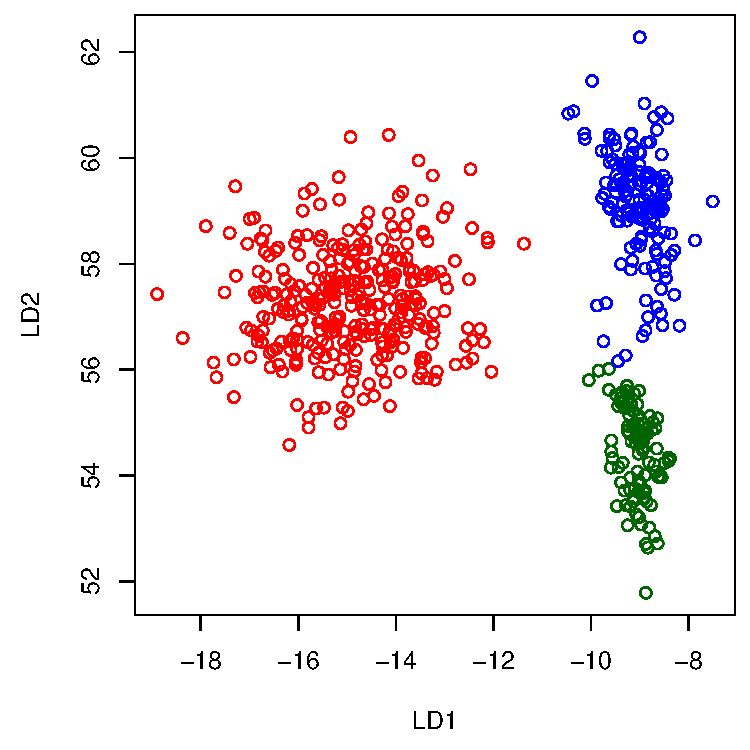
\includegraphics[width = 0.8\textwidth]{lda.pdf}
\end{center}

}

\frame{
\frametitle{Iris Data Revisited}
We next consider predicting what class each iris will be put into using QDA. The following plot is obtained.
\begin{center}
\vspace*{-.8cm}
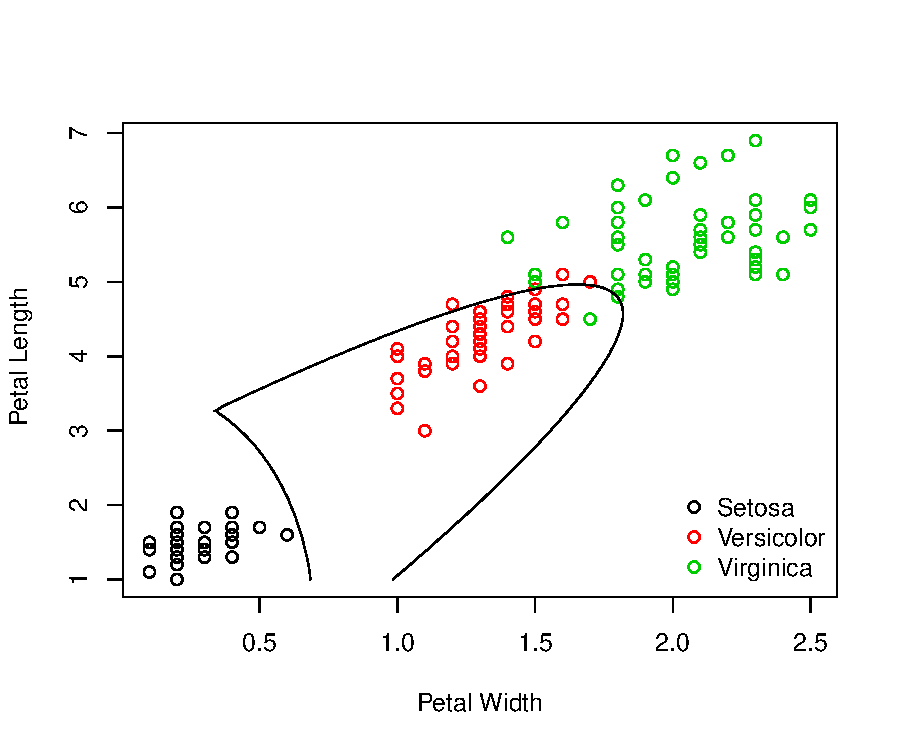
\includegraphics[width = 0.8\textwidth]{qda.pdf}
\end{center}

}





\section{Extensions}
\subsection{RDA}

\frame{
\frametitle{Regularized Discriminant Analysis}
\begin{itemize}
\item Friedman (1989) proposed a compromise between LDA and QDA.
\item This method says that we should shrink the covariance matrices of QDA toward a common covariance matrix as done in LDA.
\item Regularized covariance matrices take the form
$$ \hat{\Sigma_k}(\alpha) = \alpha\hat{\Sigma_k} + (1- \alpha)\hat{\Sigma},\quad 0 \leq \alpha \leq 1.$$
\item In practice, $\alpha$ is chosen based on performance of the model on validation data or by using cross-validation.


\end{itemize}





}

\subsection{Reduced-Rank LDA}
\frame{
\frametitle{Geometric Interpretation of LDA}
Recall $K$ is the number of classes. Consider the centers of the $K$ classes (centroids) which lie in a subspace of dimension $K$-1.
\begin{itemize}
\item We have a new observation, $\bm{x_{new}}$. For simplicity, consider $p$=2 and $K$=2.\item $\bxapp$ is defined to be the line that goes through the centroids after transforming the data to make it more spherical (ensures the line connecting the centroids is also the line that gives the greatest separation between the classes).
\item $\bxbpp$ is defined to be the line that is perpendicular to $\bxapp.$
\item After the data are transformed we will denote the new axes by $\bxap$ and $\bxbp.$




\end{itemize}
}


\frame{
\frametitle{Procedure}


\begin{enumerate}

\item Estimate the within class covariance matrix, $\hat{\Sigma} =: W$.
\item Transform the data and for each class by multiplying each data point by $W^{-1/2}.$ Also, transform $\bm{x_{new}}.$
\item Plot $\bm{x^{'}}$'s instead of $\bx$'s to get new coordinate space.
\item To classify $\bm{x_{new}}$, classify this point to the class for which $\bm{x_{new}}$ is closest to that class's centroid. 
\item $\bxapp$ is the line passing through the centroids and $\bxbpp$ is the line perpendicular to $\bxapp$ in the $p$=2, $K$=2 case.


\end{enumerate}
}

\frame{
\frametitle{Two Dimensional Example}
\begin{center}
\vspace*{-1cm}
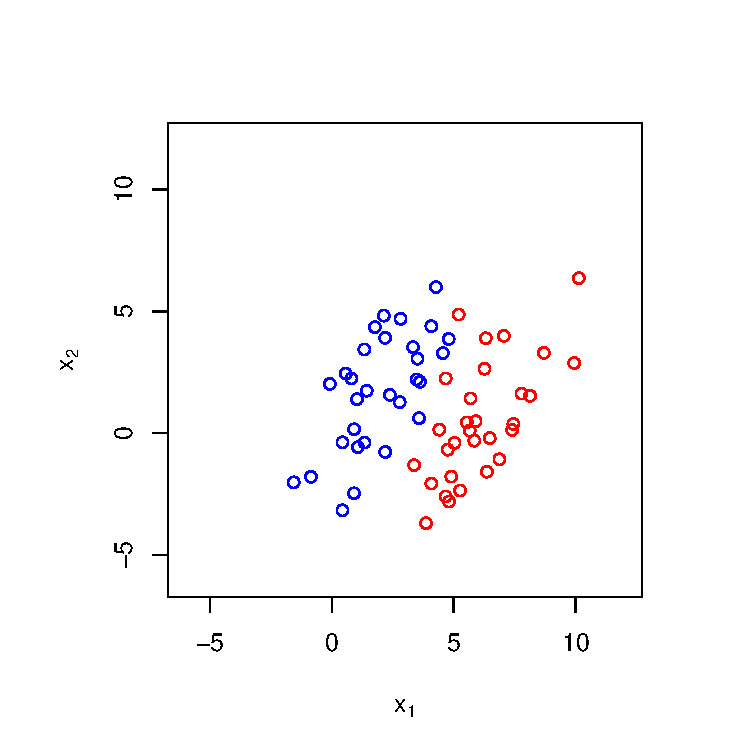
\includegraphics[width = 0.8\textwidth]{fisher.pdf}
\end{center}
}


\frame{
\frametitle{Two Dimensional Example}
\begin{center}
\vspace*{-1cm}
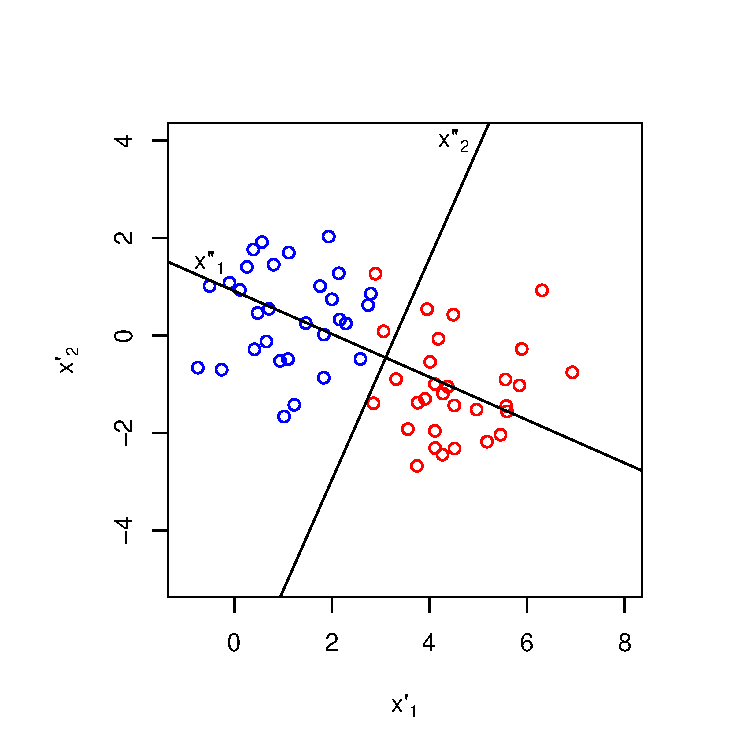
\includegraphics[width = 0.8\textwidth]{fisher_trans.pdf}
\end{center}
}

\frame{
\frametitle{Fisher's Method}
Fisher proposed an alternative derivation to dimension reduction in LDA that is equivalent to the ideas previously discussed. He suggested the proper way to rotate the coordinate axes was by maximizing the variance between classes relative to the variance within the classes.

\begin{itemize}
\item Let $Z = \ba'X$ and find the l.c. $Z$ such that the between class variance is maximized wrt within class variance.
\item Denote the covariance of the centroids by $B$.
\item Denote the pooled within class covariance  of the original data by $W$.
\item BC $\Var(Z) = \ba'B\ba$ and WC $\Var(Z) = \ba'W\ba$.
\item $B + W = T$ = total covariance matrix of $X$.
\end{itemize}
}

\frame{
\frametitle{Fisher's Method}
Fisher's problem amounts to maximizing 

$$ \max_{\ba} \frac{\ba'B\ba}{\ba'W\ba} \quad (exercise).$$ 
The solution is $\bm{a}$ = largest eigenvalue of $W^{-1}B.$\newline


Once we find the solution to maximization problem above, denoted by $\baa$, we repeat the process again of maximization except this time the new maximum, $\bab$, must be orthogonal to $\baa.$ This process continues and $\bak$ are called the discriminant coordinates. In terms of what we did earlier, the $\bak$'s are equivalent to the $\bxkpp$'s.

}




\section{Conclusions}
\frame{
\frametitle{Summary}

\begin{itemize}
\item Using linear regression to predict for indicator variables is a naive method that can lead to entire classes being masked.
\item LDA, QDA, and Regularized Discriminant Analysis procedures avoid this problem by approaching the situation with a more sound theoretical justification. 
\item Reduced-Rank LDA is desirable in high dimensions since it leads to a further dimension reduction in LDA. \newline


\end{itemize}
}










\end{document}
